%!TEX root = ../template.tex
%%%%%%%%%%%%%%%%%%%%%%%%%%%%%%%%%%%%%%%%%%%%%%%%%%%%%%%%%%%%%%%%%%%%
%% chapter2.tex
%% NOVA thesis document file
%%
%% Chapter with the template manual
%%%%%%%%%%%%%%%%%%%%%%%%%%%%%%%%%%%%%%%%%%%%%%%%%%%%%%%%%%%%%%%%%%%%

\typeout{NT FILE chapter2.tex}%

\chapter{State of the Art \& Related Work}
\label{cha:users_manual}

\glsresetall

This chapter provides a comprehensive review of the current state of the art in genomics, emphasizing the transformative role of artificial intelligence (AI) in modern DNA sequencing and analysis. It begins with an introduction to genomics as a scientific discipline, exploring the structure, function, and evolution of genomes, along with the foundational advancements enabled by projects such as the Human Genome Project. 

The chapter delves into DNA sequencing techniques, with a primary focus on Sanger sequencing, highlighting its historical significance, methodology, and key components. 

Core concepts of machine learning and deep learning are introduced in latter sections, emphasizing their application in automating and enhancing genomic analysis tasks. Important topics such as overfitting, bias-variance tradeoff, and model optimization are thoroughly discussed, reflecting the relevance of these challenges in the context of AI-driven genomics research. This chapter aims to establish a clear understanding of the foundational and emerging methodologies that define the field today.
\section{Genomics}

Genomics is the study of the structure, function, and evolution of genomes—the complete set of DNA within an organism. It encompasses various aspects, including gene identification, genome sequencing, and the analysis of genetic interactions. The field has advanced rapidly since the completion of the Human Genome Project, which mapped the entire human genome, enabling breakthroughs in personalized medicine, evolutionary biology, and disease research \cite{lander2001initial,venter2001human,genome_gov_hgp}.

Modern genomics leverages high-throughput sequencing technologies, such as next-generation sequencing (NGS), which generate vast amounts of data at unprecedented speeds. These technologies, combined with computational tools, have transformed our ability to explore genetic information on a massive scale. Genomics not only provides insights into fundamental biological processes but also underpins critical applications in biotechnology, agriculture, and healthcare \cite{metzker2010sequencing,mardis2017dna}.

\begin{figure}[H]
\centering
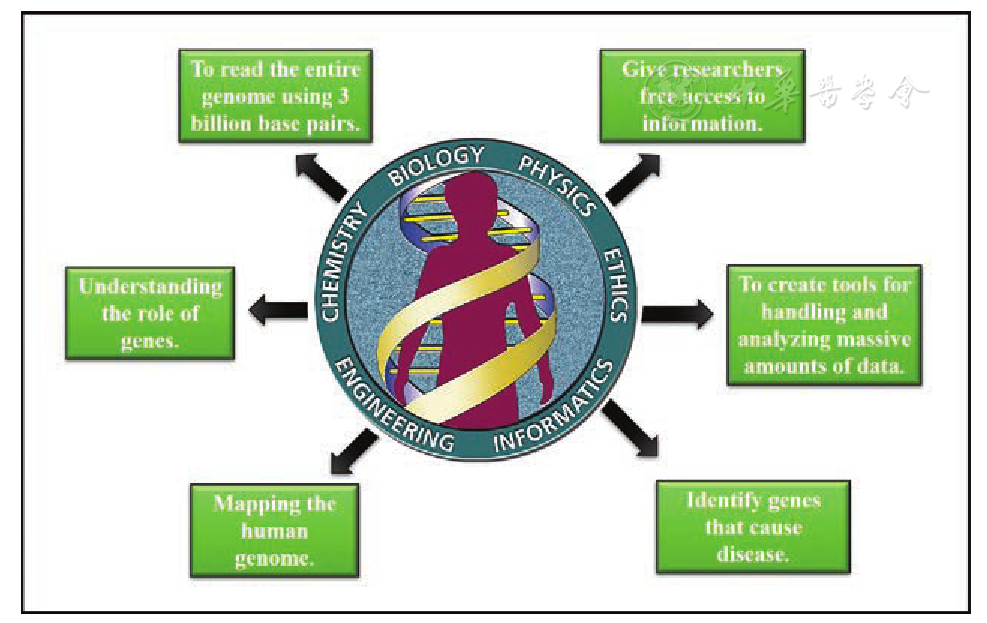
\includegraphics[width=0.8\textwidth]{hgp.png}
\caption{Objectives of Human Genome Project: The Human Genome Project was an international scientific endeavor with the aim of finding the base pairs that constitute human DNA as well as of identifying, mapping, and sequencing every gene in the human genome from both a physical and functional perspective \cite{sharma2023genetic_engineering}.}
\label{fig:hgp}
\end{figure}

\subsection{Introduction to DNA}
DNA (deoxyribonucleic acid) is the molecular blueprint for all living organisms, carrying the genetic instructions necessary for growth, development, and reproduction. The structure of DNA was famously elucidated by Watson and Crick in 1953, a discovery that revolutionized molecular biology \cite{watson_crick_dna}. DNA consists of two complementary strands coiled into a double helix, with nucleotide bases (adenine, thymine, cytosine, and guanine) forming the rungs of the helix \cite{khan_dna_structure}.

\begin{figure}[H]
\centering
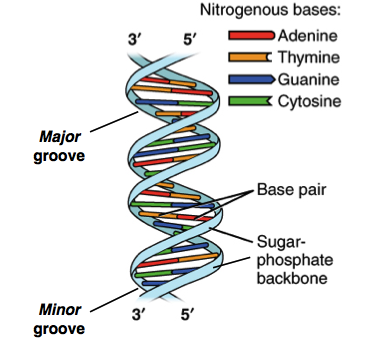
\includegraphics[width=0.5\textwidth]{dna_double_helix.png}
\caption{The structure of the DNA double helix.}
\label{fig:dna_double_helix}
\end{figure}

\subsection{DNA Sequencing and Sanger Sequencing}
DNA sequencing is the process of determining the precise order of nucleotides within a DNA molecule. Among the sequencing methods, Sanger sequencing, developed by Frederick Sanger in 1977, has long been the gold standard due to its high accuracy and reliability \cite{sanger_method_original}. This method, also known as the chain termination method, involves the selective incorporation of chain-terminating dideoxynucleotides (ddNTPs) during DNA replication, resulting in DNA fragments of varying lengths that can be analyzed to determine the DNA sequence \cite{maxam1977sequencing}.

While Sanger sequencing remains indispensable, next-generation sequencing (NGS) technologies have emerged in recent years. These technologies offer higher throughput and faster sequencing capabilities, enabling the sequencing of entire genomes quickly and cost-effectively \cite{metzker2010sequencing}. However, Sanger sequencing retains its significance for specific applications such as sequencing small, targeted regions of the genome, validating NGS results, and scenarios where longer read lengths are advantageous \cite{mardis2017dna}.

Despite advancements in NGS, Sanger sequencing continues to be favored for its simplicity, cost-effectiveness in low-throughput projects, and unparalleled accuracy. Its enduring role in genomic research and clinical diagnostics highlights its importance, particularly for applications requiring meticulous validation of genetic data \cite{shendure2017dna}.

This section explores the principles and methodologies of Sanger sequencing, emphasizing its relevance and applications in modern genomic studies.
Sequencing DNA is fundamental to understanding genetic information, enabling applications ranging from disease diagnosis and treatment to evolutionary biology \cite{turn0search0}. By deciphering the nucleotide order, scientists can identify mutations, study gene expression, and uncover genetic diversity.

To better understand the components involved in the Sanger Sequencing process:
\begin{itemize}
    \item \textbf{DNA Template}: The single-stranded DNA to be sequenced.
    \item \textbf{Primer}: A short single-stranded oligonucleotide complementary to the target sequence, serving as the starting point for DNA synthesis.
    \item \textbf{DNA Polymerase}: An enzyme that synthesizes new DNA strands by adding nucleotides to the primer.
    \item \textbf{Deoxynucleotides (dNTPs)}: Normal nucleotides (A, T, C, G) used to elongate the DNA strand.
    \item \textbf{Dideoxynucleotides (ddNTPs)}: Modified nucleotides (ddATP, ddTTP, ddCTP, ddGTP) that terminate DNA strand synthesis upon incorporation due to the lack of a 3′-OH group.
\end{itemize}

The steps of Sanger sequencing are enumerated as follows and illustrated in Figure \ref{fig:sanger_steps}: 
\begin{enumerate} 
\item \textbf{Primer annealing and chain extension}: DNA polymerase synthesizes complementary DNA strands using a primer and a mixture of deoxynucleotides (dNTPs). 
\item \textbf{ddNTP binding and chain termination}: The incorporation of ddNTPs halts DNA synthesis at specific nucleotides, resulting in DNA fragments of varying lengths. 
\item \textbf{Fluorescent labeling of DNA fragments}: The terminated DNA strands are fluorescently labeled for detection. 
\item \textbf{Capillary gel electrophoresis and fluorescence detection}: DNA fragments are separated by capillary gel electrophoresis and identified based on fluorescence signals. 
\item \textbf{Sequence analysis and reconstruction}: The nucleotide sequence is reconstructed from the fluorescence data and analyzed. 
\end{enumerate}

\begin{figure}[H]
\centering
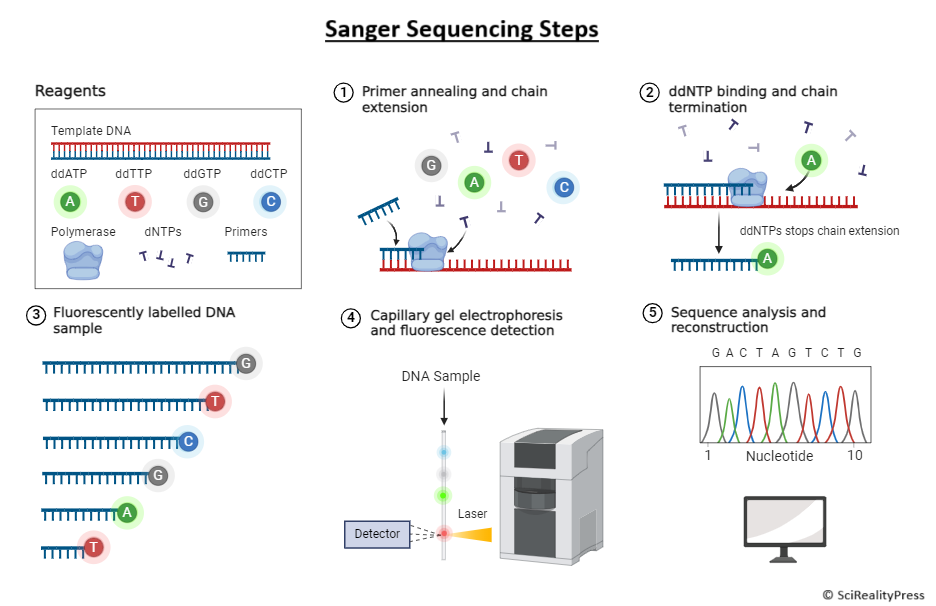
\includegraphics[width=0.9\textwidth]{sanger_steps.png}
\caption{Steps involved in Sanger sequencing \cite{biotechreality_sanger_steps}.}
\label{fig:sanger_steps}
\end{figure}

\section{Artificial Intelligence}
Artificial intelligence (AI) represents a paradigm shift in how data is analyzed and interpreted across multiple fields, including genomics. AI encompasses a broad range of computational techniques aimed at simulating human intelligence, including learning, reasoning, and self-correction \cite{russell2010artificial}. These capabilities enable AI systems to process and analyze vast amounts of data, uncover hidden patterns, and make informed predictions.
The journey of AI began with early algorithms that could perform basic logical reasoning. Over time, advancements in computational power and data availability led to the development of sophisticated methods like \textbf{Machine Learning (ML)} and \textbf{Deep Learning (DL)}, which are now at the forefront of AI innovation.
The development of AI has been greatly accelerated by advancements in computational power, data availability, and algorithmic improvements \cite{brynjolfsson2014second}. 

\subsection{Data Science}
Data is the cornerstone of achieving optimal model performance in Artificial Intelligence (AI). The effectiveness of AI models hinges on the quality and relevance of the data used for training. These models learn from the data provided, and their ability to generate accurate responses is directly tied to the insights they extract during this process. In the context of Data Science, this underscores the critical importance of data preparation, including cleaning, transformation, and feature engineering, as these steps lay the foundation for robust and reliable AI systems \cite{goodfellow2016deep,provost2013data}.
Data Science is an interdisciplinary field that combines domain expertise, programming skills, and knowledge of mathematics and statistics to extract meaningful insights from structured and unstructured data \cite{cathy2017data}. It serves as the foundation for advanced technologies like Machine Learning (ML) and Deep Learning (DL), offering essential tools and methodologies for data processing and analysis \cite{domingos2012few}. The importance of Data Science lies in its ability to bridge the gap between raw data and actionable insights. By leveraging techniques such as data cleaning, transformation, and visualization, it enables the identification of patterns, trends, and correlations that would otherwise remain hidden \cite{james2013introduction}. This process lays the groundwork for training ML and DL models by ensuring that the data is accurate, complete, and relevant.

The key components of Data Science include:
\begin{itemize}
    \item \textbf{Data Collection:} Gathering data from diverse sources, such as experiments, databases, or web scraping \cite{han2011data}.
    \item \textbf{Data Cleaning:} Addressing issues like missing values, duplicates, and inconsistencies to ensure data quality \cite{kotsiantis2006data}.
    \item \textbf{Exploratory Data Analysis (EDA):} Using statistical techniques and visualization tools to understand the underlying structure of the data \cite{tukey1977exploratory}.
    \item \textbf{Feature Engineering:} Transforming raw data into meaningful features that enhance the performance of ML models \cite{guyon2003introduction}.
    \item \textbf{Model Evaluation:} Assessing the performance of predictive models using metrics like accuracy, precision, and recall \cite{fawcett2006introduction}.
\end{itemize}

Data Science is a crucial step for ML and DL because the quality and relevance of data directly impact model performance. Poor data quality can lead to inaccurate predictions, while well-prepared data ensures that models can learn effectively and generate reliable results \cite{bishop2006pattern}.

\subsection{Machine Learning and Deep Learning}
One of the key approaches within AI is Machine Learning (ML), which has become central to modern AI development. A more specialized area within ML is Deep Learning, which utilizes neural networks with multiple layers to model and solve highly complex problems. Deep Learning is considered a subset of ML, focused on using deep neural networks to automatically learn hierarchical representations of data.

The overall structure of AI can be thought of as a hierarchy, where AI is the overarching field that encompasses various approaches, with ML being a significant subset. Within ML, Deep Learning stands as a specialized technique designed to handle large, unstructured data by leveraging multi-layered networks. This structure allows each level to address different aspects of problem-solving, with Deep Learning excelling in tasks that require high levels of abstraction and complex pattern recognition.
\begin{figure}[H]
    \centering
    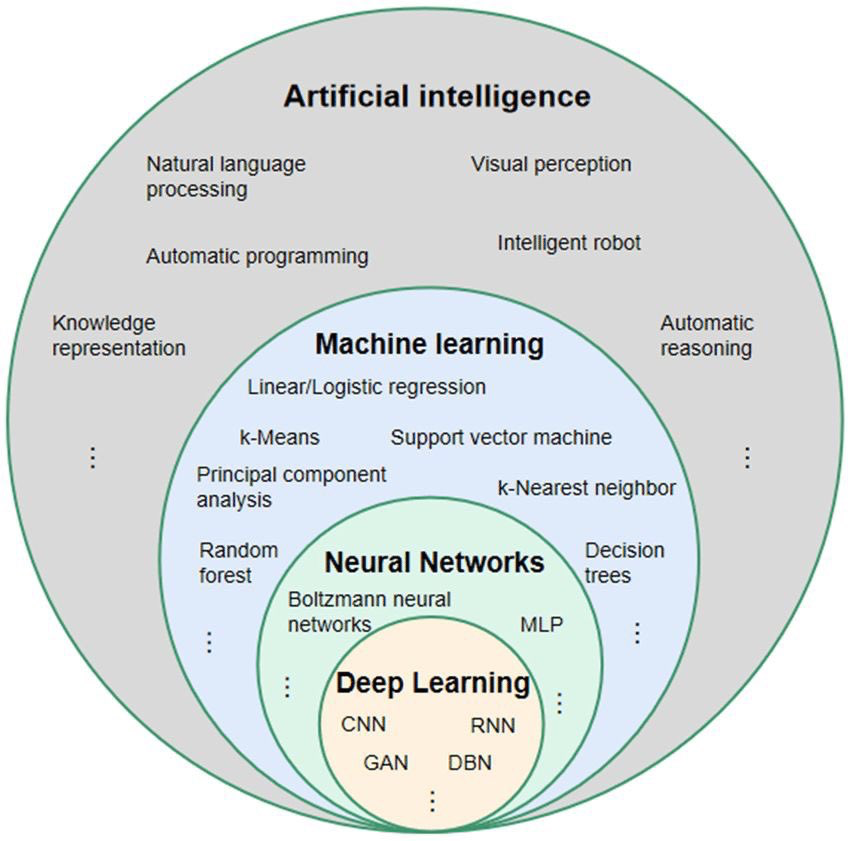
\includegraphics[width=0.7\textwidth]{ai.png}
    \caption{Understanding what Machine Learning and Deep Learning are, as subsets of Artificial Intelligence \cite{premierneurology2025image}.}
    \label{fig:ai}
\end{figure}

\subsubsection{Machine Learning}
\paragraph{Machine Learning:} Machine Learning (ML) is a subset of AI focused on developing algorithms that enable systems to learn from data and make decisions without explicit programming. In ML, algorithms are trained to recognize patterns and infer insights from large datasets \cite{bishop2006pattern}.
ML techniques are typically divided into three main categories based on the nature of the training data:
\begin{itemize} 
    \item \textbf{Supervised Learning}: The algorithm is trained on labeled data, where the input data is paired with the correct output. The goal is to learn a mapping from inputs to outputs, as seen in classification or regression tasks \cite{murphy2012machine}. 
    \item \textbf{Unsupervised Learning}: This method involves training on data that has no labels. The algorithm tries to identify hidden patterns or structures, such as grouping similar data points into clusters \cite{james2013introduction}. 
    \item \textbf{Reinforcement Learning}: The algorithm learns by interacting with its environment and receiving feedback through rewards or penalties. It is particularly useful in dynamic environments where decisions have long-term consequences \cite{sutton2018reinforcement}. 
\end{itemize}
\begin{figure}[H]
    \centering
    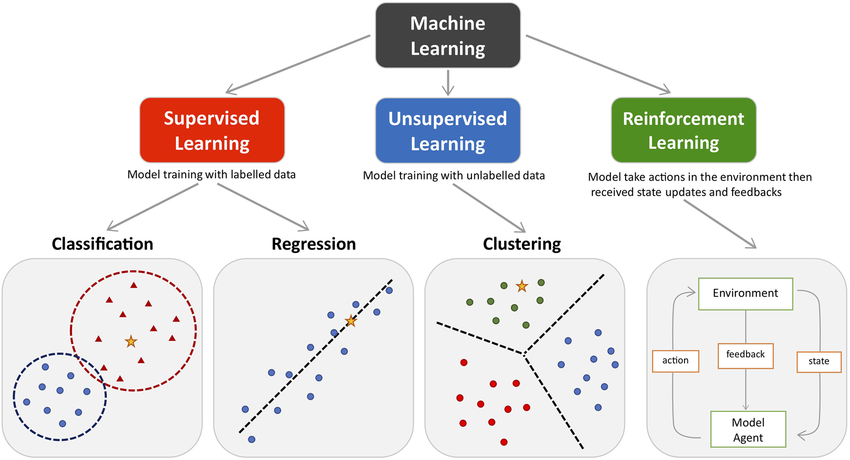
\includegraphics[width=0.7\textwidth]{ml.png}
    \caption{Illustration of the main types of Machine Learning.}
    \label{fig:ml}
\end{figure}

\subsubsection{Deep Learning}
\paragraph{Deep Learning:} Deep Learning, a specialized area of machine learning, leverages artificial neural networks with multiple layers (hence "deep") to model and solve highly complex problems. By simulating the way humans learn from data, deep learning excels in identifying patterns, handling large datasets, and making predictions with high accuracy. Key architectures in deep learning include: 
\begin{itemize}
    \item \textbf{Convolutional Neural Networks (CNNs):} CNNs are particularly effective for analyzing data with a spatial structure, such as images or signals. They have found applications in areas like object detection, image classification, and medical imaging \cite{lecun1998gradient, lecun2015deep}.
    \item \textbf{Recurrent Neural Networks (RNNs):} RNNs are designed to handle sequential data, making them well-suited for tasks like natural language processing and time series analysis. Advanced variants, such as Long Short-Term Memory networks (LSTMs) and Gated Recurrent Units (GRUs), address challenges like vanishing gradients in longer sequences \cite{hochreiter1997long, cho2014learning}.
    \item \textbf{Transformers:} Transformers revolutionized sequential data processing by introducing self-attention mechanisms, allowing the model to consider relationships between all elements in a sequence simultaneously. Transformers underpin models like BERT and GPT, which have demonstrated state-of-the-art performance in natural language understanding and generation \cite{vaswani2017attention, devlin2018bert}.
    \item \textbf{Autoencoders:} Autoencoders are unsupervised learning models that focus on efficient data encoding. They are widely used for dimensionality reduction, anomaly detection, and data denoising \cite{hinton2006reducing, vincent2010stacked}.
\end{itemize}

\begin{figure}[H]
    \centering
    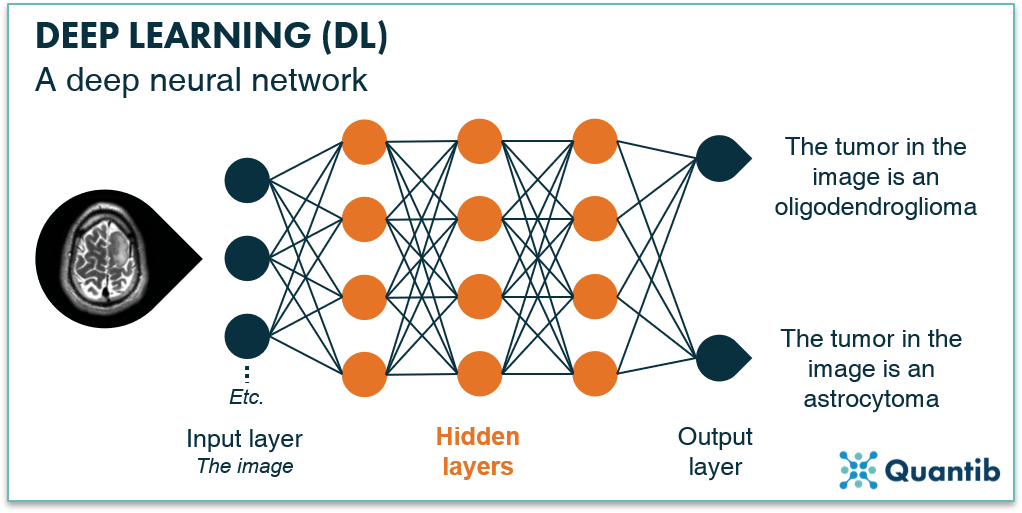
\includegraphics[width=0.5\textwidth]{dl1.png}
    \caption{A deep neural network consists of an input layer, multiple hidden layers and an output layer, all consisting of nodes \cite{quantib_deep_learning_radiology}.}
    \label{fig:dl1}
\end{figure}

\begin{figure}[H]
    \centering
    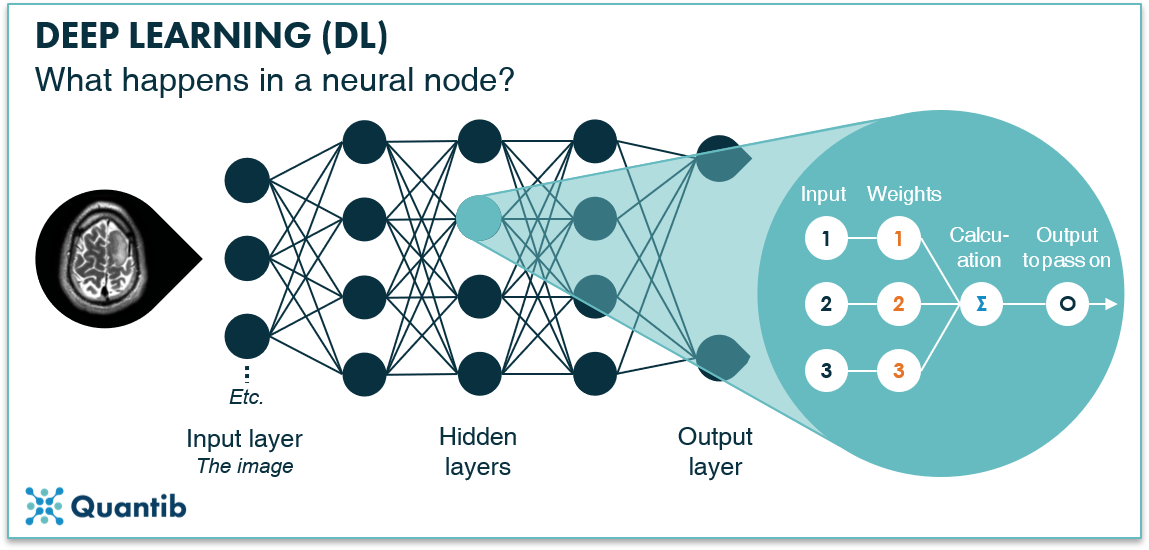
\includegraphics[width=0.5\textwidth]{dl2.png}
    \caption{A node in a hidden layer of a deep neural network takes an input, performs a calculation, and passes on an output to nodes in the next layer \cite{quantib_deep_learning_radiology}.}
    \label{fig:dl2}
\end{figure}

\begin{figure}[H]
    \centering
    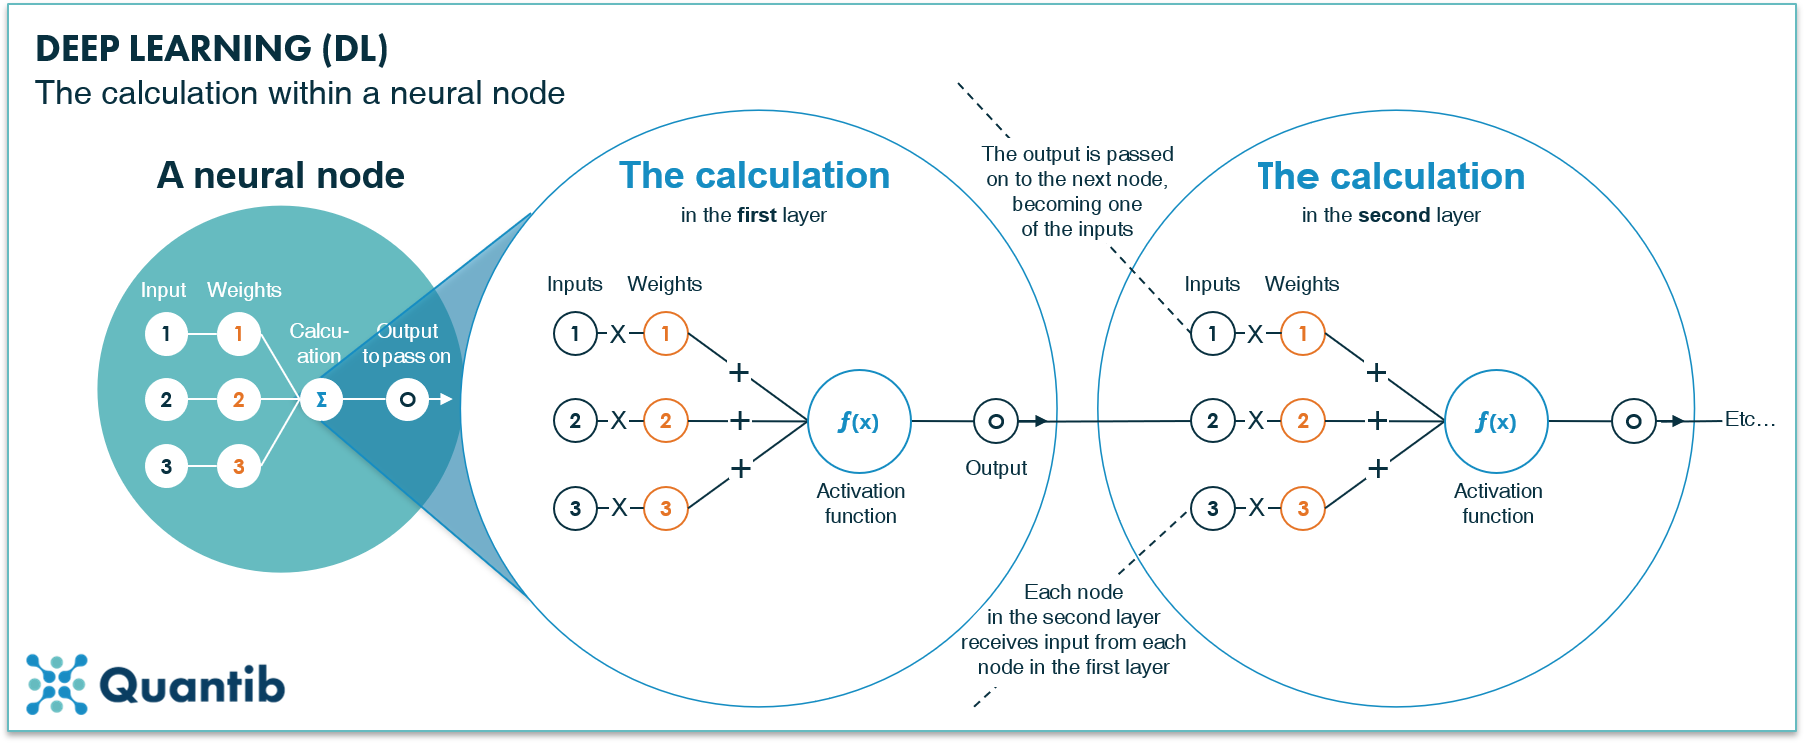
\includegraphics[width=0.5\textwidth]{dl3.png}
    \caption{Each neural node in a deep neural network performs a calculation by taking inputs from nodes in the previous layer, multiplying these by weights, and summing all outcomes. The resulting number gets processed by an activation function to allow for more complex calculations. Lastly, the output is passed on to the nodes in the next layer \cite{quantib_deep_learning_radiology}.}
    \label{fig:dl3}
\end{figure}


\subsection{Considerations for Model Selection \& Development}
Despite the vast array of deep learning techniques available, the choice of model should always align with the problem's context. Not all tasks require complex, deep networks; in fact, for simpler problems, simpler models may be more effective.

\subsubsection{Overfitting}
Overfitting is a common issue in machine learning, occurring when a model learns not only the underlying patterns in the training data but also the noise. This results in poor generalization to new, unseen data. Overfitting is particularly problematic when using overly complex models for relatively simple tasks. 

For example, handwritten digit recognition tasks (such as the MNIST dataset) can be effectively solved using shallow neural networks or simpler models like Support Vector Machines (SVMs). Using a deep architecture, such as a Convolutional Neural Network (CNN), which is more suitable for complex datasets like ImageNet, would add unnecessary complexity and increase the risk of overfitting \cite{hastie2009elements, he2016deep}.


To understand overfitting, it is essential to differentiate between training error and test error. 

\paragraph{Training Error}  refers to the error a model makes on the data it was trained on. A model that memorizes the training set perfectly will have a very low training error, but this does not necessarily mean it will perform well on new data.

\paragraph{Test Error} , on the other hand, measures the model's performance on unseen data. A well-generalized model maintains a balance between training error and test error. However, an overfitted model will exhibit a large gap between the two: it performs exceptionally well on training data but poorly on test data \cite{geman1992neural, bishop2006pattern}.

\paragraph{Causes of Overfitting} 
Overfitting is not solely caused by model complexity. Several factors contribute to this issue:

\begin{itemize}
    \item \textbf{Model Selection:} Choosing a model that is too complex for the given dataset can lead to overfitting. For instance, using a deep neural network for a simple classification problem may result in unnecessary memorization rather than pattern recognition \cite{domingos2012few}.
    \item \textbf{Insufficient Training Data:} When the dataset is too small, the model may not capture the true distribution of the data and instead learn noise as patterns. Expanding the dataset through data augmentation, synthetic data generation, or collecting more samples can mitigate this issue \cite{shorten2019survey}.
    \item \textbf{Lack of Regularization:} Regularization techniques such as L1/L2 regularization (ridge and lasso regression), dropout in neural networks, and early stopping help prevent overfitting by constraining the model’s complexity \cite{srivastava2014dropout}.
    \item \textbf{Training for Too Many Epochs:} Over-training a model without early stopping can cause it to learn noise from the training data, reducing generalization to new examples \cite{prechelt1998early}.
    \item \textbf{High Feature Dimensionality:} If a model has too many features relative to the number of training samples, it may fit noise instead of meaningful relationships. Feature selection and dimensionality reduction techniques, such as Principal Component Analysis (PCA), can help mitigate this risk \cite{jolliffe2002principal}.
\end{itemize}

\paragraph{Mitigating Overfitting} 
To reduce overfitting and improve generalization, various strategies can be employed:

\begin{itemize}
    \item \textbf{Cross-validation:} Splitting data into multiple folds for training and validation helps estimate a model's performance on unseen data \cite{kohavi1995study}.
    \item \textbf{Early stopping:} Monitoring validation loss and stopping training before overfitting occurs prevents unnecessary memorization of noise \cite{prechelt1998early}.
    \item \textbf{Regularization:} Techniques like dropout, weight decay, and batch normalization help prevent overfitting by introducing constraints \cite{srivastava2014dropout}.
    \item \textbf{Data augmentation:} Applying transformations such as rotation, scaling, and flipping to training samples increases dataset diversity and improves model robustness \cite{shorten2019survey}.
    \item \textbf{Reducing model complexity:} Choosing a simpler model that still captures essential patterns prevents unnecessary parameterization \cite{domingos2012few}.
\end{itemize}

By understanding and addressing the causes of overfitting, models can be optimized to balance training and test performance, ensuring their reliability in real-world applications.


\begin{figure}[H]
    \centering
    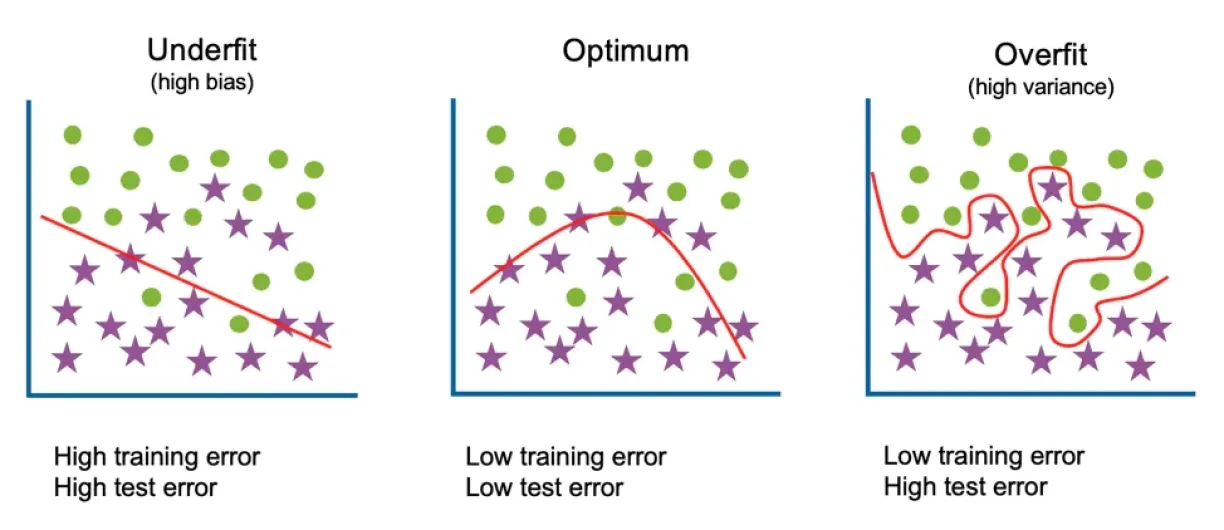
\includegraphics[width=0.9\textwidth]{overfitting.png}
    \caption{The Optimum Regression compared to Underfitting and Overfitting the prediction. \cite{aimultiple2024overfitting}.}
    \label{fig:overfitting}
    \end{figure}

\subsubsection{Balancing Bias and Variance}
Bias and variance are two fundamental sources of error in machine learning models, and understanding their trade-off is crucial for building models that generalize well to new data \cite{geman1992neural}.

\paragraph{Bias:}refers to the error introduced by approximating a real-world problem with a simplified model. A model with high bias makes strong assumptions about the data and may fail to capture the underlying patterns, leading to underfitting \cite{friedman2001elements}. This means that the model performs poorly on both training and test data. 
For example, using a linear regression model to fit a dataset with a highly nonlinear relationship would result in high bias. The model would fail to capture the complexity of the data, leading to systematic errors in its predictions \cite{friedman2001elements}.

\paragraph{Variance:}refers to the model's sensitivity to small fluctuations in the training data. A model with high variance captures noise in the training set instead of just the underlying patterns, leading to overfitting \cite{bishop2006pattern}. This results in good performance on training data but poor generalization to unseen data. 
For instance, a deep neural network with a large number of parameters trained on a small dataset may memorize the training data but fail to generalize. The model's high variance means it is too dependent on the specifics of the training data, leading to poor performance on unseen samples \cite{bishop2006pattern}.

\paragraph{The Trade-Offs:} The trade-off between bias and variance is fundamental when selecting a model. Simpler models, such as linear regression or decision trees, generally exhibit higher bias but lower variance. These models are often preferable for tasks with limited data or when interpretability is critical. On the other hand, more complex models like Gradient Boosted Machines (GBMs) or neural networks tend to have lower bias but higher variance. Regularization techniques are often employed to control overfitting in these cases \cite{bishop2006pattern, domingos2012few}.
The goal of machine learning is to find a balance between bias and variance to minimize total error. A model with high bias and low variance tends to underfit, while a model with low bias and high variance tends to overfit. The optimal trade-off ensures that the model has just the right complexity to generalize well \cite{domingos2012few}. Regularization techniques, cross-validation, and careful model selection help manage this trade-off effectively.


\begin{figure}[H]
    \centering
    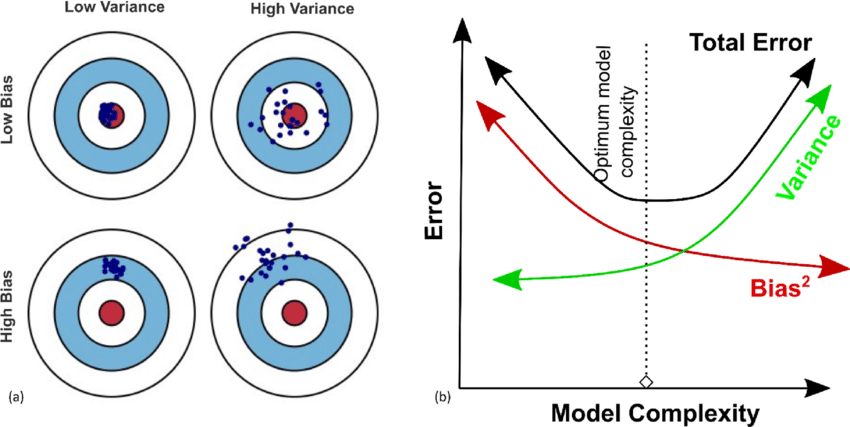
\includegraphics[width=0.9\textwidth]{biasvariance.png}
    \caption{(a) Graphical illustration of bias and variance. The aim is to obtain a model that has low bias and low variance. (b) Contribution of bias and variance to the total error of the machine learning model (reproduced from the reference [57]). With increasing model complexity, error function reduced significantly for training data set but perform poorly in validation dataset, i.e., higher variance. The task to define a model in such a way that the bias and variance can tackle in validation and blind test data set. \cite{bias_variance_illustration}.}
    \label{fig:biasvariance}
    \end{figure}

\subsubsection{Occam's Razor for Model Selection \& Simplicity}
Occam's razor \cite{britannica_occams_razor} serves as a guiding principle: among competing models, the simplest one that adequately explains the data should be preferred. For instance, Pedro Domingos highlights the importance of understanding when complexity adds value and when it merely adds noise \cite{domingos2012few}.
By adhering to this principle, one can avoid unnecessary complexity and focus on building models that are both effective and efficient.

\subsubsection{Conclusion}

In the context of machine learning and deep learning, choosing the right model depends on the specific problem, available data, and computational resources. While complex models like deep neural networks are powerful, they should be used judiciously. For many tasks, simpler models may offer equal or better performance with fewer risks of overfitting, lower computational costs, and greater interpretability. A thoughtful approach to model selection ensures that the chosen algorithm is both efficient and appropriate for the task at hand.

\section{Related Work}
Artificial Intelligence (AI) techniques have revolutionized genomics by enabling automation and optimization of DNA analysis processes. This chapter examines AI-driven methods closely related to the scope of this thesis, which focuses on automating the quarantining of DNA wells in a 96-well plate format. Two studies are discussed in depth, followed by a comparative analysis.
The application of AI in genomics spans clustering, classification, and anomaly detection. Among these, two notable works are:

\begin{enumerate}
    \item \textbf{DeepConsensus: Deep Learning for DNA Sequence Correction}: This study leverages convolutional neural networks (CNNs) to correct errors in raw DNA sequences, improving downstream analysis \cite{deepconsensus}.
    \item \textbf{ClusterGAN: Semi-Supervised Clustering for Genomic Data}: This method combines generative adversarial networks (GANs) with clustering to group similar genomic sequences while mitigating the need for extensive labeled data \cite{clustergan}.
\end{enumerate}

\subsection{DeepConsensus: Deep Learning for DNA Sequence Correction}

This study introduces a deep learning framework, DeepConsensus, designed to enhance the accuracy of raw DNA sequences obtained from sequencers.

\textbf{Key Features:}
\begin{itemize}
    \item \textbf{Model Architecture:} Employs convolutional neural networks (CNNs) to learn patterns of errors in sequencing data.
    \item \textbf{Input Data:} Raw sequencing reads, encoded numerically for model compatibility.
    \item \textbf{Output:} Corrected sequences that improve downstream processes like alignment and variant calling.
\end{itemize}

\textbf{Strengths:}
\begin{itemize}
    \item Substantial reduction in sequencing errors.
    \item Applicability across different sequencer technologies.
    \item Improved data quality for downstream genomic applications.
\end{itemize}

\textbf{Limitations:}
\begin{itemize}
    \item High computational cost for training deep models.
    \item Requires large datasets for optimal performance.
\end{itemize}

\subsection{ClusterGAN: Semi-Supervised Clustering for Genomic Data}

ClusterGAN combines generative adversarial networks (GANs) with clustering objectives to categorize genomic data with minimal supervision.

\textbf{Key Features:}
\begin{itemize}
    \item \textbf{Architecture:} Incorporates a generator and discriminator, alongside a clustering head for unsupervised grouping.
    \item \textbf{Input Data:} Encoded genomic sequences in a numerical format.
    \item \textbf{Output:} Clusters of genomic sequences based on similarity.
\end{itemize}

\textbf{Strengths:}
\begin{itemize}
    \item Effectively handles unlabeled genomic data.
    \item Learns latent representations of sequences for clustering.
    \item Adaptable to various types of genomic datasets.
\end{itemize}

\textbf{Limitations:}
\begin{itemize}
    \item GAN training can be unstable.
    \item Limited interpretability of learned latent features.
\end{itemize}

\subsection{Comparison with Current Work}

A comparison between these related works and the approach of this thesis is summarized in Table \ref{tab:comparison}.

\begin{table}[h]
\centering
\caption{Comparison of Related Works with Thesis Approach}
\label{tab:comparison}
\begin{tabular}{|l|l|l|l|}
\hline
\textbf{Aspect}              & \textbf{DeepConsensus}               & \textbf{ClusterGAN}                  & \textbf{Thesis Approach}             \\ \hline
Algorithm                    & CNN-based Error Correction           & GAN-based Clustering                 & Similarity-Based Quarantining        \\ \hline
Data Type                    & Raw Sequencing Reads                 & Encoded Genomic Sequences            & Numerical Data (e.g., concentrations, IDs) \\ \hline
Supervision                  & Fully Supervised                     & Semi-Supervised                      & Unsupervised                        \\ \hline
Output                       & Corrected DNA Sequences              & Clusters of Genomic Sequences        & Cluster and Quarantine Visualization  \\ \hline
Scalability                  & Moderate                             & High                                 & High                                 \\ \hline
Computational Cost           & High                                 & High                                 & Moderate                             \\ \hline
\end{tabular}
\end{table}

\subsection{Conclusion}

While DeepConsensus and ClusterGAN significantly contribute to error correction and clustering in genomic data, this thesis addresses a unique challenge: automating the quarantining process of DNA wells in 96-well plates. By integrating clustering and domain-specific constraints, the proposed method ensures practical applicability in genomic laboratories, enhancing scalability and robustness.